\section{Exercise 2 - Implement Linear Pipeline for \texttt{MPI\_Bcast} and \texttt{MPI\_Reduce}}

SLIDES ZITIERN, PAPER TRAEFF ZITIERN, REFERENZ ZU NER ANDEREN CHAPTER MACHEN

The goal of exercise 2 is to implement linear pipelined versions of \texttt{MPI\_Bcast()} and \texttt{MPI\_Reduce()} 
based on the algorithms discussed in the lecture (refer to Algorithm 16 and Algorithm 17 of "Algorithms for Collective 
Communication"). \\

Our implementation for the pipelined reduction -- \texttt{MY\_Reduce\_P()} – aligns with the following idea: We 
distinct between a master process (rank $= 0$), interior processes ($0 <$ rand $<$ size $-1$) and an end process 
(rank $=$ size $-1$). As an output of \texttt{MY\_Reduce\_P()}, the master shall possess the entry-wise maximum as 
reduction result. Additionally, we divide the array that needs to be compared into multiple blocks of size 
\texttt{blockSize} (and probably a smaller block in the end). Goal is to communicate between the processes for each 
block separately. \\

The end process (rank $=$ size $-1$) sends blocks – one after the other -- to the interior process with 
rank $=$ size $-2$. The end process does not receive data, as there are no further processes. Interior processes 
first receive a data block from their neighbor with rank $+1$, perform a local reduction and send this data to their 
other neighbor with rank $-1$. This is repeated for all blocks. The master process receives block data from the interior 
node of rank $=1$.\\

Our implementation for the pipelined broadcast -- \texttt{MY\_Bcast\_P()} – is quite similar to the 
\texttt{MY\_Reduce\_P()} implementation. For broadcast the goal is that the data which is I the beginning 
available for the master process shall be communicated to all the other processes. In order to do so, the master 
process sends its data block wise to its neighbor with rank $=1$ (interior process). Interior processes receive block 
data from their predecessor process and immediately communicate this data to their successor process – block by 
block. The last one to receive the data is the end processor. There is no need to send any further data from here.\\

The trivial combination of \texttt{MY\_Reduce\_P()} and \texttt{MY\_Bcast\_P()} can be seen as a pipelined variant 
of \texttt{MPI\_Allreduce()}.\\

\begin{figure}[h]
\begin{center}
    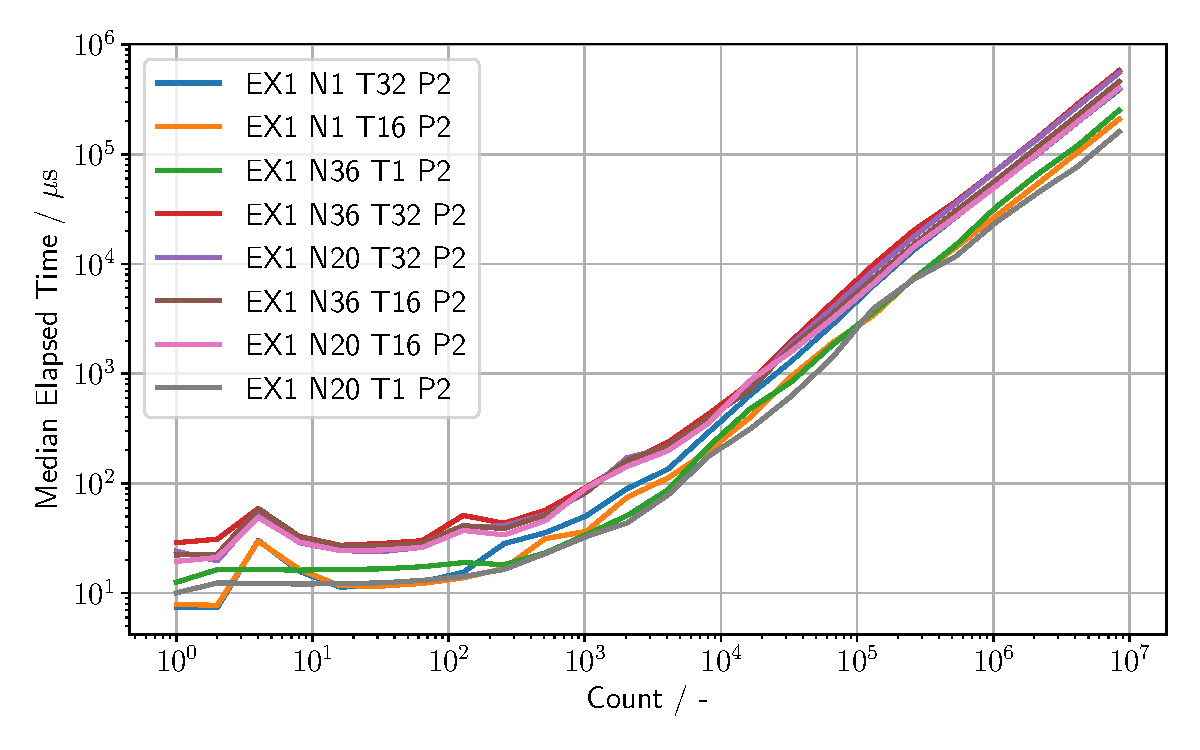
\includegraphics[width=1.0\linewidth]{figures/Ex2_1.pdf}
    \caption{Caption for Ex2 plot 1}
    \label{Ex2_1_p}
\end{center}
\end{figure}

\begin{figure}[h]
\begin{center}
    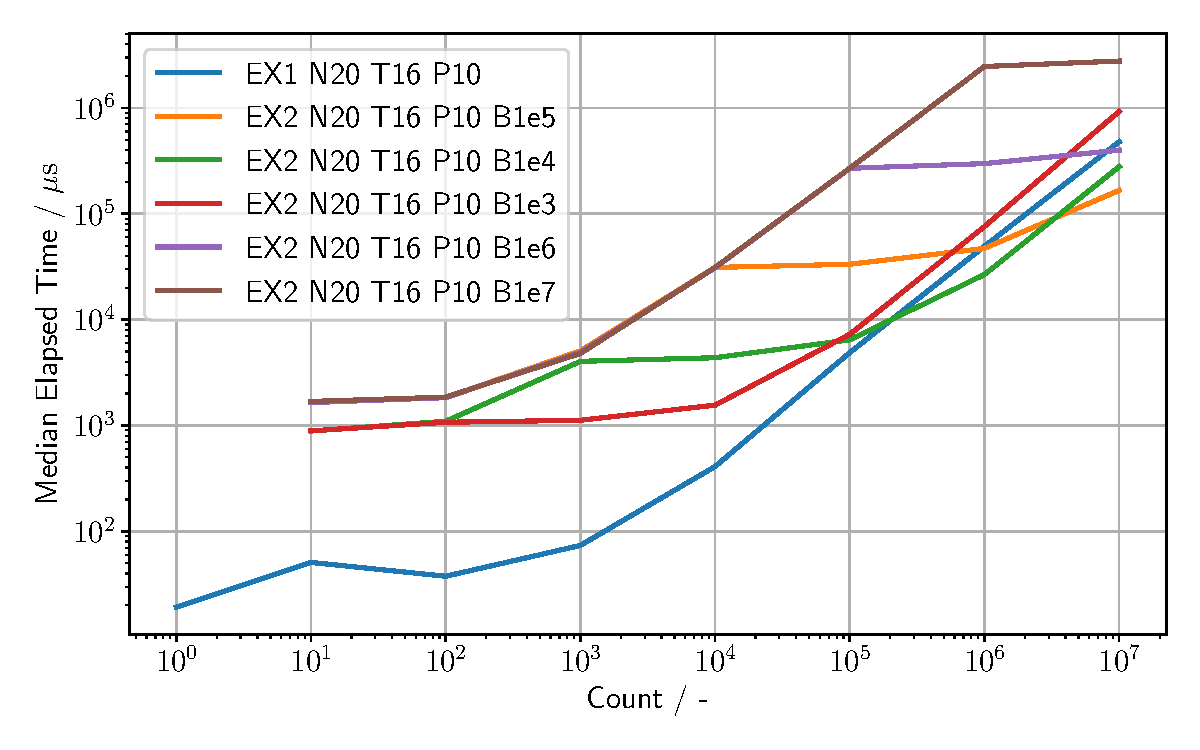
\includegraphics[width=1.0\linewidth]{figures/Ex2_2.pdf}
    \caption{Caption for Ex2 plot 2}
    \label{Ex2_2_p}
\end{center}
\end{figure}

\begin{figure}[h]
\begin{center}
    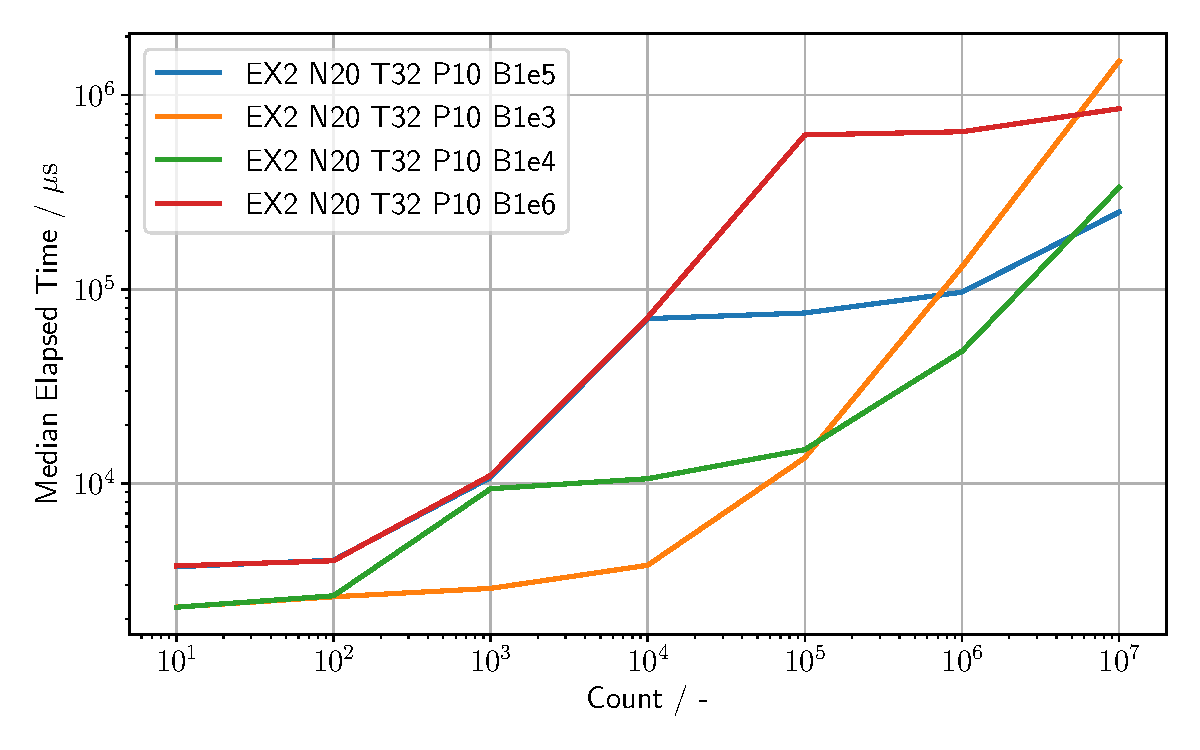
\includegraphics[width=1.0\linewidth]{figures/Ex2_3.pdf}
    \caption{Caption for Ex2 plot 3}
    \label{Ex2_3_p}
\end{center}
\end{figure}

%% 2_4 and 2_5 plots next to each other!

\begin{figure}[h]
\centering
    \begin{minipage}{.5\textwidth}
        \centering
        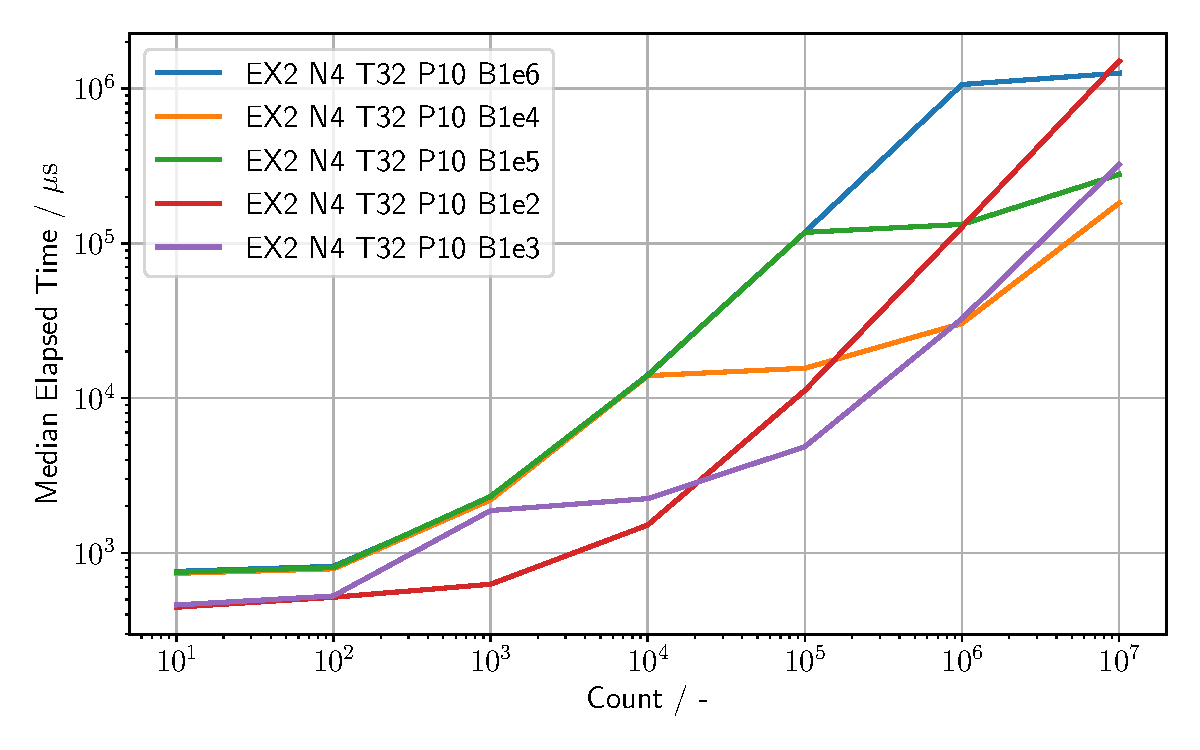
\includegraphics[width=1.0\linewidth]{figures/Ex2_4.pdf}
        \captionof{figure}{Caption for Ex2 plot 4}
        \label{Ex2_4_p}
    \end{minipage}%
    \begin{minipage}{.5\textwidth}
        \centering
        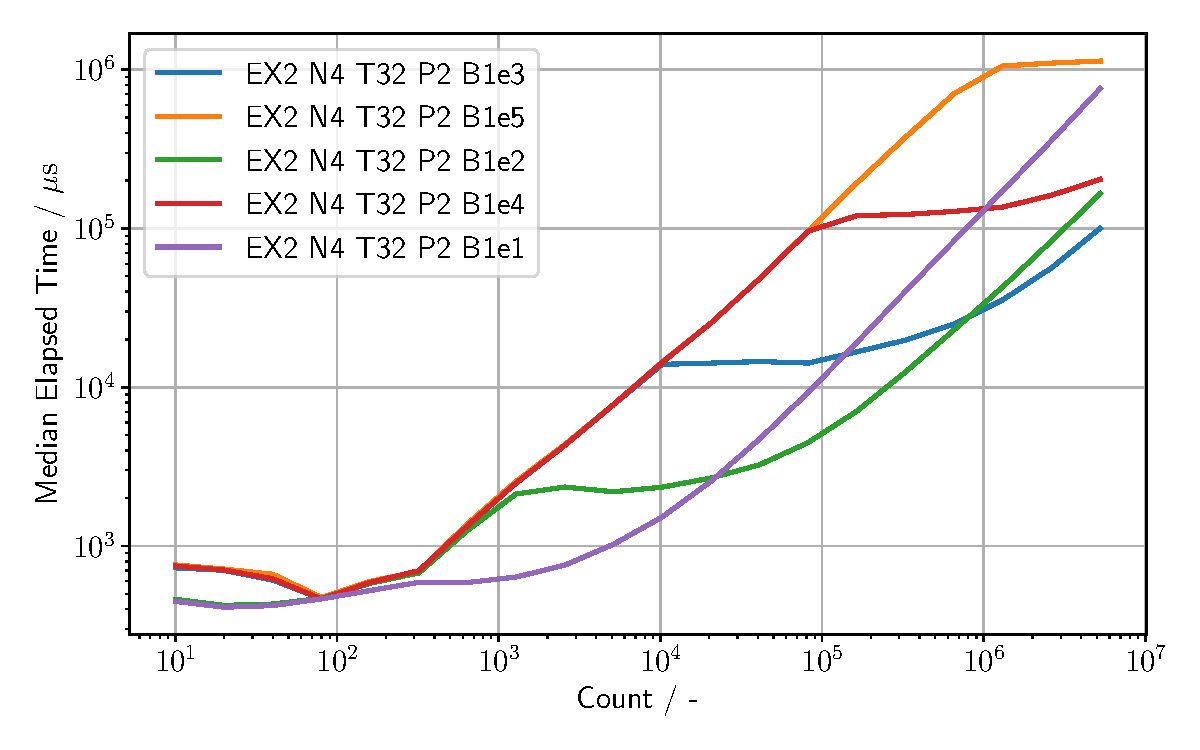
\includegraphics[width=1.0\linewidth]{figures/Ex2_5.pdf}
        \captionof{figure}{Caption for Ex2 plot 5}
        \label{Ex2_5_p}
    \end{minipage}
\end{figure}

% \begin{figure}[h]
%     \begin{center}
%         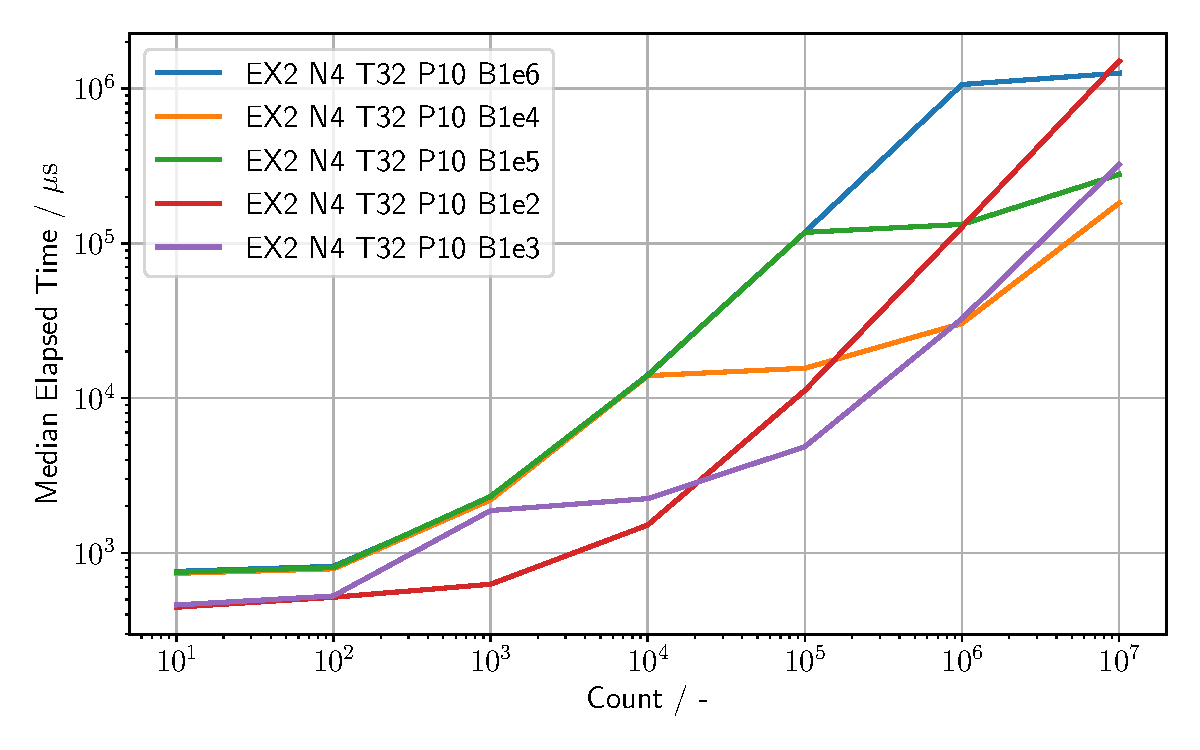
\includegraphics[width=1.0\linewidth]{figures/Ex2_4.pdf}
%         \caption{Caption for Ex2 plot 4}
%         \label{Ex2_4_p}
%     \end{center}
% \end{figure}

% \begin{figure}[h]
%     \begin{center}
%         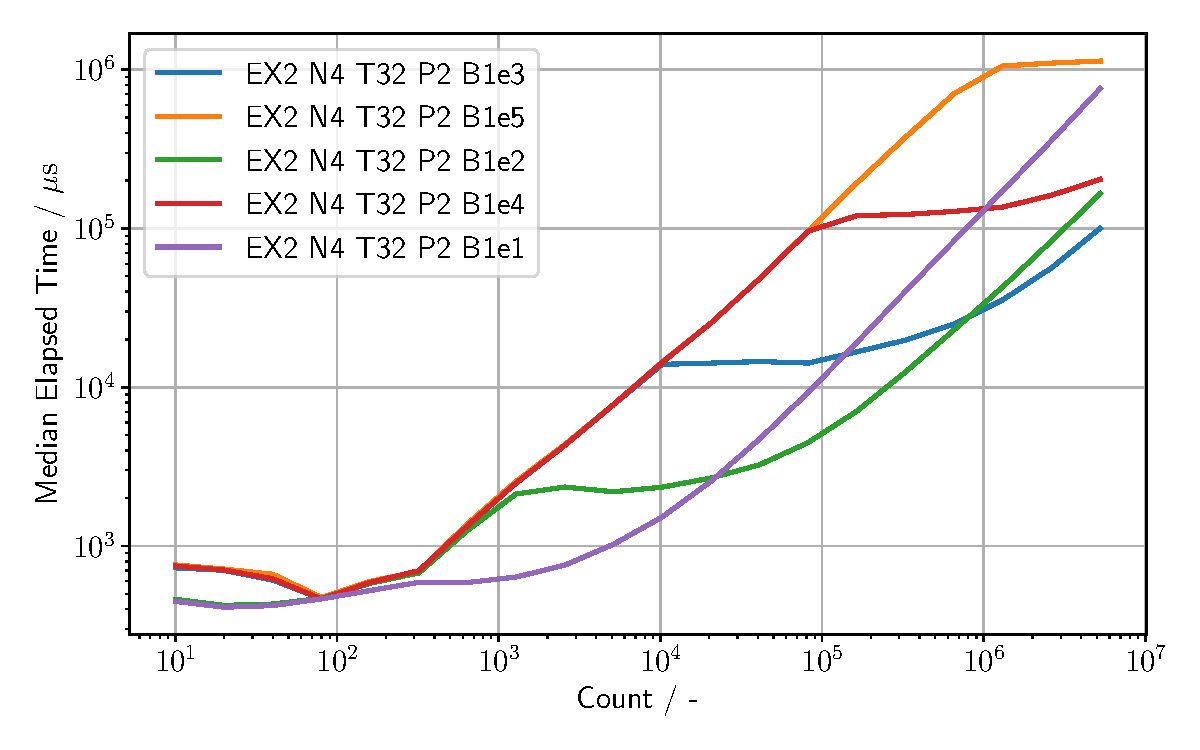
\includegraphics[width=1.0\linewidth]{figures/Ex2_5.pdf}
%         \caption{Caption for Ex2 plot 5}
%         \label{Ex2_5_p}
%     \end{center}
% \end{figure}


